\documentclass[notheorems]{beamer} % option notheorems
\usepackage[utf8]{inputenc}
\usepackage[main=russian,english]{babel}
\usepackage{amsfonts,amsmath,amssymb,amsthm}
\usepackage{algorithm,algpseudocode}

\usetheme{Madrid}
\usecolortheme{default}

\newtheorem{definition}{Определение}
\newtheorem{examples}{Примеры}

\newcommand{\w}{\textbf{w}}
\newcommand{\x}{\textbf{x}}

\DeclareMathOperator*{\argmax}{argmax}
%------------------------------------------------------------
%This block of code defines the information to appear in the
%Title page
\title[Теоретические основы  ML] %optional
{Градиентный спуск \\ Нейронные сети}

%\author {Б.В.В.}



\date[Теория игр] % (optional)
{Теория игр,  2023}

\logo{
\includegraphics[height=1cm]{MIREA_logo}}

%End of title page configuration block
%------------------------------------------------------------



%------------------------------------------------------------
%The next block of commands puts the table of contents at the 
%beginning of each section and highlights the current section:

\AtBeginSection[]
{
  \begin{frame}
    \frametitle{Содержание}
    \tableofcontents[currentsection]
  \end{frame}
}
%------------------------------------------------------------


\begin{document}

%The next statement creates the title page.
\frame{\titlepage}


%---------------------------------------------------------
%This block of code is for the table of contents after
%the title page
\begin{frame}
\frametitle{Содержание}%-------------------------------------
\tableofcontents
\end{frame}
%---------------------------------------------------------
\section{Машинное обучение с учителем}

%---------------------------------------------------------
\begin{frame}
	\frametitle{Используемая литература}
\begin{itemize}
	\item Christopher Bishop. Pattern Recognition and Machine Learning
	\item Shai Shalev-Shwartz, Shai Ben-David. Understanding Machine Learning: From Theory to Algorithms
	\item Jorge Nocedal, Stephen J. Wright. Numerical Optimization
\end{itemize}	






	
\end{frame}
%---------------------------------------------------------
%---------------------------------------------------------
\begin{frame}
	\frametitle{ Машинное обучение с учителем }
	
	
	Множество объектов  $\mathcal{X}=\{\textbf{x} \}$ , представленных вектором из  $d$ признаков $\textbf{x}=(x_1, \dots,x_d)$
	
	Множество значений зависимой переменой $\mathcal{Y}=\{y \}$  
	
	Множество моделей(гипотез) $\mathcal{H}$, описываемых в виде функции, которая каждому объекту ставит в соответствие одно  значений зависимой переменой $h: \mathcal{X} \to \mathcal{Y}$.
	
	Функция потерь $ \ell:\mathcal{H} \times \mathcal{X} \times \mathcal{Y} \to \mathbb{R_+}$
	
\end{frame}
%---------------------------------------------------------
\begin{frame}
	\frametitle{Истинная ошибка }
	
	
	Множество объектов  $\mathcal{X}=\{\textbf{x} \}$ , представленных вектором из  $d$ признаков $\textbf{x}=(x_1, \dots,x_d)$
	
	Множество значений зависимой переменой $\mathcal{Y}=\{y \}$  
	
	Множество моделей(гипотез) $\mathcal{H}$, описываемых в виде функции, которая каждому объекту ставит в соответствие одно  значений зависимой переменой $h: \mathcal{X} \to \mathcal{Y}$.
	
	Функция потерь $ \ell:\mathcal{H} \times \mathcal{X} \times \mathcal{Y} \to \mathbb{R_+}$
	
	При заданном \alert{вероятностном распределении $\mathcal{D}$ над $ \mathcal{X}\times\mathcal{Y} $} функция $ \ell $ является случайной
	\begin{block}{Истинная ошибка модели $ h \in \mathcal{H} $ }
		математическое ожидание функции потери  модели  $ h $:
		$$L_D(h) = \mathop{\mathbb{E}}_{(\textbf{x},y)\sim\mathcal{D}} [\ell(h(\textbf{x}),y)] $$ 
	\end{block}
	
\end{frame}

%---------------------------------------------------------
\begin{frame}
	\frametitle{Эмпирическая ошибка}
	
	
	Множество объектов  $\mathcal{X}=\{x \}$ , представленных вектором из  $d$ признаков $\mathbf{x}=(x_1, \dots,x_d)$
	
	Множество значений зависимой переменой $\mathcal{Y}=\{y \}$  
	
	Множество моделей(гипотез) $\mathcal{H}$, описываемых в виде функции, которая каждому объекту ставит в соответствие одно  значений зависимой переменой $h: \mathcal{X} \to \mathcal{Y}$.
	
	Функция потерь $ \ell:\mathcal{H} \times \mathcal{X} \times \mathcal{Y} \to \mathbb{R_+}$
	
	Так как в большинстве случаев распределение $\mathcal{D}$ неизвестно, то модель выбирается по \alert{имеющейся выборке из $m$ объектов $$ S =  ((\textbf{x}^{(1)},y^{(1)}), \dots, (\textbf{x}^{(m)}, y^{(m)}))$$ }
	
	
	\begin{block}{Эмпирическая ошибка модели $ h \in \mathcal{H} $ }
		\begin{equation}
		\label{eqn:emp_risk}
		L_S(h) = \frac{1}{m}\sum_{i=1}^{m} \ell(h(\textbf{x}^{(i)}),y^{(i)}) 
		\end{equation}
	\end{block}
	
\end{frame}

%---------------------------------------------------------

%---------------------------------------------------------
\begin{frame}
	\frametitle{Задача регрессии}
	
	
	Множество объектов  $\mathcal{X}=\{\textbf{x} \}$ , представленных вектором из  $d$ признаков $\textbf{x}=(x_1, \dots,x_d)$
	
	Множество значений зависимой переменой $\mathcal{Y}=\alert{\mathbb{R}}$  
	
	Множество моделей(гипотез) $\mathcal{H}$, описываемых в виде функции, которая каждому объекту ставит в соответствие одно  значений зависимой переменой $h: \mathcal{X} \to \mathcal{Y}$.
	
	Функция потерь $ \ell:\mathcal{H} \times \mathcal{X} \times \mathcal{Y} \to \mathbb{R_+}$
	
	\alert{$ h,\textbf{x},y \mapsto (h(\textbf{x})-y)^2$}
	
\end{frame}
%---------------------------------------------------------
\begin{frame}
	\frametitle{Пример задачи регрессии}
	Объект задается набором (вектором) $d$ признаков $\textbf{x}=(x_1, ..., x_d)$
	Модель - линейная функция от вектора параметров $\textbf{w}$
	$$h_{\textbf{w}}(\textbf{x})=h(\textbf{x}, \textbf{w})=w_0 + x_1*w_1 + ... +x_d*w_d=\langle \textbf{x},\textbf{w} \rangle  $$
	\begin{columns}
		\begin{column}{.5\linewidth}\centering
			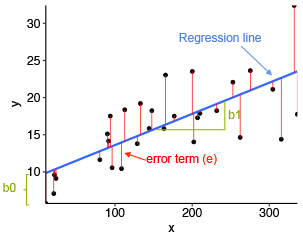
\includegraphics[width=0.8\textwidth]{img/linear_regression}
		\end{column}
		\begin{column}{.5\linewidth}\centering
			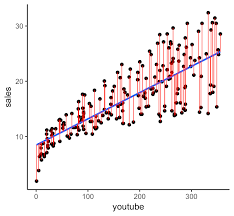
\includegraphics[width=0.8\textwidth]{img/lr_youtube}
	\end{column}
	\end{columns}
\end{frame}
%---------------------------------------------------------
\begin{frame}
	\frametitle{Задача классификации}
	
	
	Множество объектов  $\mathcal{X}=\{x \}$ , представленных вектором из  $d$ признаков $\mathbf{x}=(x_1, \dots,x_d)$
	
	Множество значений зависимой переменой $\mathcal{Y}=\alert{y_1, \dots, y_n}$  
	
	Множество моделей(гипотез) $\mathcal{H}$, описываемых в виде функции, которая каждому объекту ставит в соответствие одно  значений зависимой переменой $h: \mathcal{X} \to \mathcal{Y}$.
	
	Функция потерь $ \ell:\mathcal{H} \times \mathcal{X} \times \mathcal{Y} \to \mathbb{R_+}$
	
	\alert{$      \ell(h(\textbf{x}),y) \mapsto
		\begin{cases}
		1, & \text{если}\ h(\textbf{x})\neq y \\
		0, & \text{иначе}
		\end{cases} $}
	
\end{frame}

\begin{frame}
	\frametitle{Пример задачи классификации}
	Объект задается набором (вектором) $d$ признаков $\textbf{x}=(x_1, ..., x_d)$
	Множество значений зависимой переменой - два класса $\mathcal{Y}=\{0,1\}$
	Модель - логистическая функция от вектора параметров $\textbf{w}$
	$$h_{\textbf{w}}(\textbf{x})=h(\textbf{x}, \textbf{w})=\frac{1}
	{1 + e^{\langle \textbf{x}, \textbf{w}\rangle}}, \langle \textbf{x},\textbf{w} \rangle = w_0 + x_1*w_1 + ... +x_d*w_d  $$
	
	$$ y^{\text{гипотеза}} =		\begin{cases}
	1, & \text{если} \ h_{\textbf{w}}(\textbf{x}) >0.5 \\
	0, & \text{иначе}
	\end{cases}$$
			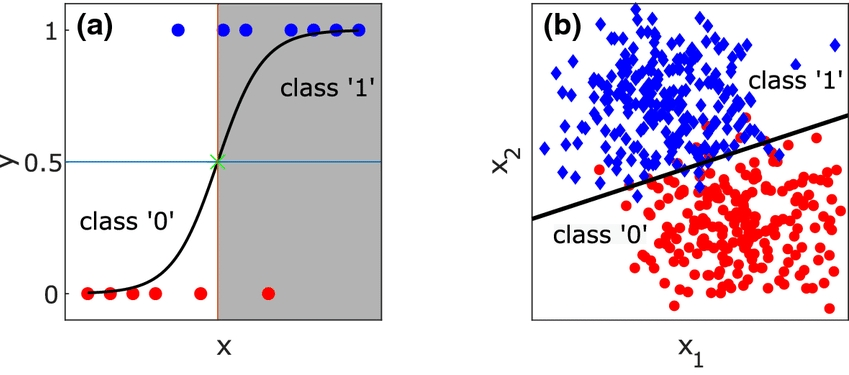
\includegraphics[width=0.75\textwidth]{img/classification_example}
\end{frame}
%---------------------------------------------------------


\section{Градиентный спуск}
%---------------------------------------------------------
%---------------------------------------------------------
\begin{frame}
	\frametitle{Задача оптимизации}
	Минимизация эмпирической ошибки модели $ h \in \mathcal{H} $ 
	\begin{equation}
	L_S(h_{\textbf{w}}) = L_S(\textbf{w}) = \frac{1}{m}\sum_{i=1}^{m} \ell(h(\textbf{x}^{(i)}, \textbf{w}),y^{(i)})  \to \min_{\textbf{w}}
	\end{equation}
	
		\begin{block}{Общая постановка задачи оптимизации для произвольной функции 	
				$f: \mathbb{R}^n \to \mathbb{R}$				
			}
		\begin{equation}
		f(\textbf{w})   \to \min_{\textbf{w}}
		\end{equation}
	\end{block}
	$\w*$ - минимум функции $f$, если $\forall \w\ f(\w^*) \leq f(\w)$
\end{frame}
%---------------------------------------------------------
\begin{frame}
	\frametitle{Градиент}
	
	$f: \mathbb{R}^n \to \mathbb{R}$
	
	$\w \mapsto f(\w)$
	
	\begin{block}{Градиент функции $f$ в точке $p$ }
		$\nabla f: \mathbb{R}^n \to \mathbb{R}^n$ 
		
	
		$$
		\nabla f_{\w}(p)=\left[\begin{array}{c}
		\dfrac{\partial f}{\partial w_1}(p)\\
		\dfrac{\partial f}{\partial w_2}(p) \\
		\vdots \\
		\dfrac{\partial f}{\partial w_n}(p) 
		\end{array}\right]
		$$
		
	\end{block}
	
	

	
\end{frame}


\begin{frame}
	\frametitle{Градиентный спуск}
	
	Нахождение локального минимуму функции $f: \mathbb{R}^n \to \mathbb{R}$
	
	\begin{block}{Алгоритм }
		Инициализация $\w^0$ произвольно
		
		Для каждой итерации 
		
		выбор шага обновления $\alpha$
		$$ \w^{k+1} \leftarrow \w_{k}-\alpha\nabla f(\w_k) $$

		
	\end{block}

Для минимума $w^*$ верно $\nabla f(\w^*)=0$

\end{frame}

\section{Искусственная нейронная сеть}
%---------------------------------------------------------
\begin{frame}
	\frametitle{Нейрон}
	https://cs231n.github.io
	
		\begin{columns}
		
		\column{0.5\textwidth}
		\begin{figure}
	\includegraphics[width=1.0\textwidth]{neuron}
\end{figure}
		
		\column{0.5\textwidth}
		\begin{figure}
			\includegraphics[width=1.0\textwidth]{neuron_model}
		\end{figure}
	\end{columns}
\end{frame}

%---------------------------------------------------------
\begin{frame}
	\frametitle{Нейронная сеть}

		\begin{figure}
			\includegraphics[width=1.0\textwidth]{neural_net2}
		\end{figure}
\end{frame}
%---------------------------------------------------------
\begin{frame}
	\frametitle{Алгоритм обратного распространения}
	
	\begin{figure}
		\includegraphics[width=1.0\textwidth]{nn-calculation}
	\end{figure}
\end{frame}

\end{document}
%---------------------------------------------------------
\begin{frame}
	\frametitle{Алгоритм обратного распространения}
	
	\begin{figure}
		\includegraphics[width=1.0\textwidth]{pytorch}
	\end{figure}
\end{frame}

\end{document}